\documentclass[11pt,a4paper,twocolumn]{article}

% === Core Packages ===
\usepackage[margin=2cm]{geometry}
\usepackage[utf8]{inputenc}
\usepackage[T1]{fontenc}
\usepackage{times}
\usepackage{amsmath,amssymb}
\usepackage{graphicx}
\usepackage{booktabs}
\usepackage{float}
\usepackage{enumitem}
\usepackage{tikz}
\usepackage{pgfplots}
\pgfplotsset{compat=1.18}
\usetikzlibrary{arrows.meta,shapes.geometric,positioning,calc,decorations.markings,fit,backgrounds}

% === Citation (IEEE style) ===
\usepackage[numbers,sort&compress]{natbib}
\bibliographystyle{IEEEtranN}

% === Hyperref ===
\usepackage[hidelinks]{hyperref}
\usepackage{xurl}

% === Settings ===
\setlength{\parindent}{1em}
\setlength{\parskip}{0.3em}

% === Title ===
\title{\textbf{Decentralizovaná reputačná sieť:\\Rámec pre prirodzenú organizáciu spoločnosti}}
\author{Pavel Kudrna\\Prague, Czechia\\Draft v1 --- March 2026}
\date{}

\begin{document}
\maketitle

% ============================================================
% ABSTRACT
% ============================================================
\begin{abstract}
Zmysel pre spravodlivosť---presvedčenie, že krivdy sú napravené a zásluhy odmenené---je najsilnejšou súdržnou silou spoločnosti. Keď centralizované inštitúcie správy nedokážu tento zmysel poskytnúť, pretože náklady na vymáhanie práva prevyšujú hodnotu samotného práva, spoločenská súdržnosť sa rozpadá. Súčasné inštitucionálne štruktúry zlyhávajú pri riešení významnej triedy sporov systematicky rovnakým spôsobom, akým centrálne plánovanie zlyháva pri alokácii zdrojov: prostredníctvom informačnej asymetrie, chýbajúcich spätnoväzbových slučiek a odpojenia rozhodovateľov od dôsledkov ich rozhodnutí. Tento článok predstavuje Reputačnú sociálnu sieť (RSN): decentralizovanú, neskorumpovateľnú, voči cenzúre odolnú komunikačnú vrstvu postavenú na decentralizovaných identifikátoroch (DID), ktorá umožňuje pseudonymným účastníkom publikovať, overovať a konzumovať reputačné informácie o správaní v reálnom svete. Základný mechanizmus spočíva na troch návrhových princípoch: (1)~asymetrická nákladová štruktúra, kde čítanie reputačných dát je lacné, ale zápis vyžaduje overiteľné úsilie; (2)~nedeterministický protokol výberu overovateľa založený na konzistentnom hashovaní, ktorý oceňuje radikálne tvrdenia prostredníctvom eskalujúcich nákladov iterácií; a (3)~trhovo riadený model reputačnej autority, kde súkromní overovatelia stavajú svoju nahromadenú reputáciu na presnosť tvrdení, ktoré potvrdzujú. Výsledná architektúra produkuje emergentnú meritokraciu bez centrálnej koordinácie a umožňuje postupnú, zvratnú migračnú cestu z existujúcich štátom spravovaných systémov.
\end{abstract}

% ============================================================
% 1. INTRODUCTION
% ============================================================
\section{Úvod}

\subsection{Problém centralizovanej dôvery}

Moderná správa spoločnosti spočíva na základnom predpoklade: že centralizované inštitúcie dokážu sprostredkovať dôveru medzi neznámymi ľuďmi vo veľkom rozsahu. Súdy rozhodujú spory. Registre potvrdzujú vlastníctvo. Regulačné orgány vymáhajú štandardy. Tieto inštitúcie boli navrhnuté v čase, keď informácie boli vzácne, komunikácia bola pomalá a delegovanie autority na centrálny orgán bolo jediným uskutočniteľným koordinačným mechanizmom. Centralizovaná správa však zlyháva z rovnakých štrukturálnych dôvodov ako centrálne plánovanie: informačná asymetria, chýbajúce spätnoväzbové slučky a odpojenie rozhodovateľov od dôsledkov ich rozhodnutí.

Tento predpoklad zlyháva napríklad vtedy, keď náklady na inštitucionálne sprostredkovanie prevýšia hodnotu sporu. Uvažujme o nájomníkovi, ktorý zistí, že jeho prenajatý byt nemá zákonom vyžadovaný certifikát o elektrickej bezpečnosti---stav, ktorý predstavuje bezprostredné ohrozenie života. Zákonné právo nájomníka odstúpiť od zmluvy je jednoznačné. Náklady na vymáhanie tohto práva prostredníctvom súdneho systému však prevyšujú peňažnú hodnotu zálohy a dlžnej náhrady škody, dokonca aj vrátane možného zákonného odškodnenia~\cite{czcourtfees}. Racionálnou reakciou je stratu vstrebať a odísť.

Nejde o patologický okrajový prípad. Je to štandardná skúsenosť pre významnú triedu sporov, v ktorých je ujma reálna, ale peňažná výška klesá pod prah, pri ktorom sa inštitucionálne vymáhanie stáva ekonomicky racionálnym. Výsledkom je systém, ktorý štrukturálne zvýhodňuje zlých aktérov: tí, ktorí poškodzujú druhých v objemoch pod týmto prahom, môžu konať beztrestne, pretože náklady na dosiahnutie spravodlivosti nesie poškodená strana.

Vyššie uvedený príklad je čerpaný z autorovho právneho prostredia---českého systému občianskeho práva. V iných právnych tradíciách---precedenčnom obyčajovom práve (common law), zvykovom práve, zmiešaných systémoch---spravodlivosť zlyháva odlišnými spôsobmi a v rôznej miere, v závislosti od kultúrnych a procesných špecifík danej jurisdikcie. Čitatelia pravdepodobne rozpoznajú ekvivalentné príklady zo svojho vlastného kontextu. Štrukturálne univerzálny je vzorec: spory, ktorých hodnota klesá pod prah ekonomicky racionálneho vymáhania, končia tým, že stratu vstrebe poškodená strana. RSN nesľubuje dokonalú spravodlivosť---iba znižuje štrukturálnu výhodu, ktorú zlí aktéri požívajú, keď je inštitucionálne vymáhanie neekonomické.

\subsection{Prečo existujúce riešenia nestačia}

\textbf{Rámce decentralizovanej identity (DID)}~\cite{did2022} poskytujú kryptografické mechanizmy pre správu suverénnej identity (self-sovereign identity), ale zameriavajú sa predovšetkým na overovanie identity bez riešenia širšej otázky reputácie správania.

\textbf{Soulbound tokeny (SBT)}~\cite{weyl2022} zachytávajú poznatok, že reputácia je neprenosná, ale spoliehajú sa na blockchainovú infraštruktúru s obmedzeniami škálovateľnosti a neriešia ekonomické stimuly upravujúce vkladanie informácií. Súvisiace koncepty ako zásluhové tokeny (napr. Liberland) zdieľajú podobnú filozofiu, no zostávajú viazané na konkrétne jurisdikčné rámce.

\textbf{Decentralizované autonómne organizácie (DAO)}~\cite{buterin2014} implementujú správu prostredníctvom smart kontraktov, ale replikujú plutokratickú dynamiku, kde je vplyv úmerný kapitálu. Kvadratické hlasovanie~\cite{buterin2019} to čiastočne zmierňuje, ale obmedzuje praktické prijatie. DAO tiež čelia zásadnému \emph{problému orákula}: smart kontrakty nedokážu spoľahlivo overiť stavy reálneho sveta bez dôveryhodného externého zdroja a tento problém nemá v rámci blockchainovej architektúry všeobecné riešenie.

Žiadny existujúci systém nekombinuje decentralizáciu, odolnosť voči cenzúre, pseudonymitu, overiteľné náklady na vstup a emergentný konsenzus.

\subsection{Prínosy}

Tento článok prináša nasledujúce prínosy:
\begin{enumerate}[nosep]
\item Definíciu \textbf{Reputačnej sociálnej siete (RSN)}, decentralizovaného protokolu rozširujúceho rámec DID o podporu obojstrannej výmeny reputácie.
\item \textbf{Nedeterministický protokol výberu overovateľa} založený na konzistentnom hashovaní~\cite{karger1997}.
\item \textbf{Princíp drahého radikalizmu}, ktorý oceňuje tvrdenia podľa ich vzdialenosti od sieťového konsenzu prostredníctvom troch kumulujúcich sa nákladových kanálov.
\item Model \textbf{reputovanej autority} s asymetrickými stimulmi, kde falošné potvrdenie stojí katastrofálne viac než legitímne poplatky.
\item \textbf{Postupnú migračnú cestu} prostredníctvom paralelnej fiškálnej infraštruktúry.
\end{enumerate}

% ============================================================
% 2. DESIGN PRINCIPLES
% ============================================================
\section{Návrhové princípy}

Architektúra RSN je obmedzená piatimi nespochybniteľnými návrhovými princípmi.

\textbf{Kontinuita a evolúcia.} Systém koexistuje s existujúcimi inštitúciami počas prechodného obdobia neurčitej dĺžky. Prechod musí byť v každej fáze zvratný.

\textbf{Dobrovoľnosť a zodpovednosť.} Účasť je dobrovoľná, ale dobrovoľnosť je spojená so zodpovednosťou: účastník, ktorý preberá kontrolu nad inštitucionálnou funkciou, súčasne preberá aj sprievodné povinnosti.

\textbf{Rozmanitosť a kultúrna neutralita.} Konsenzus vzniká z obojstranných interakcií, nie z vopred stanovených pravidiel vnútených návrhármi systému.

\textbf{Odolnosť a odolnosť voči cenzúre.} Náklady na cenzurovanie siete musia prevýšiť náklady na jej tolerovanie. Iba úplný totalitarizmus---za rujnujúcich politických a ekonomických nákladov---dokáže systém potlačiť.

\textbf{Konsenzus a vymáhanie.} Systém zahŕňa ľudské sklony k malichernosti, zlomyseľnosti a odplatnému zadosťučineniu ako nosné prvky. Pochybenie nie je zakázané; je ocenené.

% ============================================================
% 3. SYSTEM OVERVIEW
% ============================================================
\section{Prehľad systému}

\subsection{Reputačná sociálna sieť}

RSN je decentralizovaná, peer-to-peer komunikačná vrstva, v ktorej si účastníci vymieňajú overiteľné informácie o správaní v reálnom svete. Jej definujúcimi vlastnosťami sú: decentralizovaná a necenzurovateľná infraštruktúra; pseudonymná účasť prostredníctvom DID; asymetrická nákladová štruktúra (čítanie je lacné, zápis je drahý); kryptografická overiteľnosť; a \textbf{podpora štandardov}---strojovo čitateľné formáty pre informácie šírené sieťou, pre služby ponúkané autoritami (skladanie tvrdení, potvrdzovanie, svedecká služba) a pre formát politiky vrátane pravidiel na hodnotenie reputácie protistrany a posudzovanie rizika nesúladu politiky (medzi deklarovaným a skutočným správaním).

\subsection{Architektonické komponenty}

RSN pozostáva zo štyroch primárnych komponentov (Obr.~\ref{fig:architecture}):
\begin{enumerate}[nosep]
\item \textbf{Vrstva DID.} Identity účastníkov s deklarovanými pravidlami, reputačnými metadátami a sieťovým smerovaním.
\item \textbf{Protokol tvrdení.} Štruktúrovaný formát na publikovanie výrokov o udalostiach v reálnom svete.
\item \textbf{Overovacia sieť.} Decentralizovaný protokol na prideľovanie overovateľov pomocou konzistentného hashovania.
\item \textbf{Vrstva agregácie reputácie.} Služby, ktoré produkujú ľudsky čitateľné súhrny reputácie.
\end{enumerate}

\begin{figure}[ht]
\centering
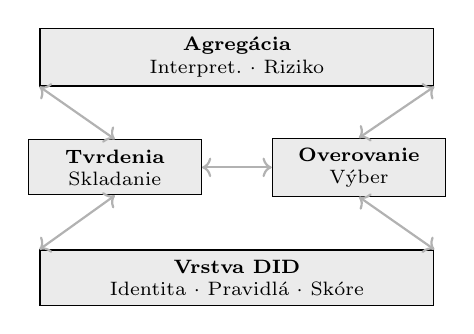
\begin{tikzpicture}[
    layer/.style={draw, minimum height=0.7cm, align=center, font=\scriptsize, fill=black!8},
    arr/.style={<->, thick, gray!60}
]
\node[layer, minimum width=5cm] (agg) at (0,2.8) {\textbf{Agregácia}\\Interpret.\ $\cdot$ Riziko};
\node[layer, minimum width=2.2cm] (claim) at (-1.55,1.4) {\textbf{Tvrdenia}\\Skladanie};
\node[layer, minimum width=2.2cm] (verif) at (1.55,1.4) {\textbf{Overovanie}\\Výber};
\node[layer, minimum width=5cm] (did) at (0,0) {\textbf{Vrstva DID}\\Identita $\cdot$ Pravidlá $\cdot$ Skóre};

\draw[arr] (agg.south west) -- (claim.north);
\draw[arr] (agg.south east) -- (verif.north);
\draw[arr] (claim.east) -- (verif.west);
\draw[arr] (claim.south) -- (did.north west);
\draw[arr] (verif.south) -- (did.north east);
\end{tikzpicture}
\caption{Štvorvrstvová architektúra RSN.}
\label{fig:architecture}
\end{figure}

\subsection{Roly účastníkov}

Overovacia transakcia zahŕňa až šesť odlišných rolí DID (Obr.~\ref{fig:roles}): \textbf{Vydavateľ} ($DID_I$, vytvára a odosiela tvrdenie), \textbf{Subjekt} ($DID_S$, DID, o ktorom tvrdenie je---môže sa zhodovať s vydavateľom), \textbf{Autorita} ($DID_A$, potvrdzuje tvrdenie za poplatok; môže tiež ponúkať svedecké služby---\emph{voliteľné}), \textbf{Svedok} ($DID_{W_{1..n}}$, inkognito monitor čestnosti overovateľa prostredníctvom výzvových kódov---\emph{voliteľné}), \textbf{Overovateľ} ($DID_V$, algoritmicky vybraný na publikovanie tvrdenia) a \textbf{RSN} (sieť, kde sa overené tvrdenia publikujú). Ktorákoľvek rola môže byť delegovaná na iný DID (kapitola~7.4). Autorita bežne zväzuje potvrdzovanie so svedeckými službami, ale obe funkcie sú logicky nezávislé.

\begin{figure}[ht]
\centering
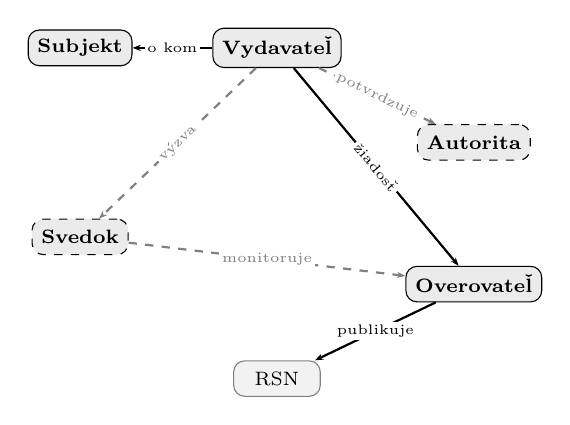
\begin{tikzpicture}[
    role/.style={draw, rounded corners, minimum width=1.1cm, minimum height=0.45cm, align=center, font=\scriptsize, fill=black!8},
    opt/.style={draw, rounded corners, minimum width=1.1cm, minimum height=0.45cm, align=center, font=\scriptsize, fill=black!8, dashed},
    arr/.style={-{Stealth[length=3pt]}, thick},
    oarr/.style={-{Stealth[length=3pt]}, thick, dashed, gray},
    lbl/.style={font=\tiny, fill=white, inner sep=1pt}
]
\node[role] (I) at (0,2.4) {\textbf{Vydavateľ}};
\node[role] (S) at (-2.5,2.4) {\textbf{Subjekt}};
\node[opt] (A) at (2.5,1.2) {\textbf{Autorita}};
\node[opt] (W) at (-2.5,0) {\textbf{Svedok}};
\node[role] (V) at (2.5,-0.6) {\textbf{Overovateľ}};
\node[role, fill=black!5, draw=gray] (N) at (0,-1.8) {RSN};

\draw[arr] (I) -- node[lbl] {o kom} (S);
\draw[oarr] (I) -- node[lbl,sloped] {potvrdzuje} (A);
\draw[oarr] (I) -- node[lbl,sloped] {výzva} (W);
\draw[arr] (I) -- node[lbl,sloped] {žiadosť} (V);
\draw[oarr] (W) -- node[lbl] {monitoruje} (V);
\draw[arr] (V) -- node[lbl] {publikuje} (N);
\end{tikzpicture}
\caption{Roly DID v overovacej transakcii. Prerušovane = voliteľné (Autorita, Svedok).}
\label{fig:roles}
\end{figure}

\subsection{Neskorumpovateľnosť: štyri sily}

Neskorumpovateľnosť RSN nevychádza z jediného mechanizmu, ale zo štyroch súčasne pôsobiacich síl. Žiadna sama osebe nepostačuje; iba ich kombinácia robí pokus o korupciu ekonomicky iracionálnym.

\textbf{Nepredvídateľný cieľ.} Overovateľ pre každé tvrdenie je vybraný nedeterministicky prostredníctvom konzistentného hashovania (kapitola~5.3). Útočník nemôže vopred zacieliť konkrétneho overovateľa na úplatok, pretože identita overovateľa je funkciou obsahu tvrdenia a predchádzajúcich iterácií, nie voľby vydavateľa.

\textbf{Reputačná páka---pomaly hore, rýchlo dole.} Reputáciu možno získať iba postupne, prostredníctvom trvalého konzistentného správania. Možno ju však stratiť katastrofálne jediným podvodným potvrdením (kapitola~6.2). Táto asymetria znamená, že roky nahromadenej reputácie môžu byť zničené jediným nečestným potvrdením; optimálnou stratégiou zostáva odmietať podozrivé tvrdenia.

\textbf{Verejný sľub.} Každý držiteľ DID verejne deklaruje svoju politiku---strojovo čitateľnú sadu pravidiel, ktoré sa zaväzuje dodržiavať. Odchýlka medzi deklaráciou a skutočným správaním je zistiteľná a ocenená ako reputačný priestupok závažnejší než samotné porušenie (kapitola~7.3). Pokrytectvo je preto nákladnejšie než priama nečestnosť.

\textbf{Asymetria nákladov na útok voči sieti (mesh).} Náklady na cenzurovanie alebo destabilizáciu siete rastú nelineárne s veľkosťou a hustotou siete, zatiaľ čo náklady na jej tolerovanie zostávajú konštantné. Aby sa cenzúra vyplatila, centralizovaný aktér by ju musel aplikovať naprieč celou sieťou---čo si vyžaduje opatrenia neúmerné akémukoľvek predstaviteľnému prospechu (kapitola~10).

% ============================================================
% 4. DECENTRALIZED IDENTITY MODEL
% ============================================================
\section{Model decentralizovanej identity}

\subsection{DID so špeciálnymi vlastnosťami}

RSN rozširuje špecifikáciu W3C DID Core~\cite{did2022} o: \textbf{deklarované pravidlá} (strojovo čitateľné záväzky týkajúce sa správania), \textbf{reputačné metadáta} (agregované skóre správania) a \textbf{sieťové smerovanie} (meniteľná onion brána oddelená od stabilnej pozície na kruhu).

\subsection{Životný cyklus tvrdenia}

Tvrdenie prechádza šiestimi fázami (Obr.~\ref{fig:lifecycle}): skladanie, voliteľné potvrdenie autoritou, výber overovateľa cez konzistentné hashovanie, rozhodnutie o overení (prijatie alebo odmietnutie s iteráciou), publikovanie a aktualizácia reputácie pre všetky strany.

\begin{figure}[ht]
\centering
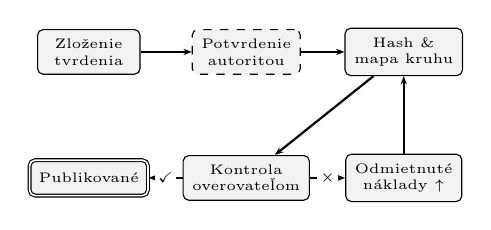
\begin{tikzpicture}[
    stp/.style={draw, rounded corners=2pt, minimum width=1.3cm, minimum height=0.45cm, align=center, font=\tiny, fill=black!5},
    arr/.style={-{Stealth[length=3pt]}, thick},
    lbl/.style={font=\tiny, fill=white, inner sep=1pt}
]
\node[stp] (comp) at (0,0) {Zloženie\\tvrdenia};
\node[stp, dashed] (auth) at (2.0,0) {Potvrdenie\\autoritou};
\node[stp] (hash) at (4.0,0) {Hash \&\\mapa kruhu};
\node[stp] (ver) at (2.0,-1.6) {Kontrola\\overovateľom};
\node[stp, double] (pub) at (0,-1.6) {Publikované};
\node[stp] (rej) at (4.0,-1.6) {Odmietnuté\\náklady $\uparrow$};

\draw[arr] (comp) -- (auth);
\draw[arr] (auth) -- (hash);
\draw[arr] (hash) -- (ver);
\draw[arr] (ver) -- node[lbl] {\checkmark} (pub);
\draw[arr] (ver) -- node[lbl] {$\times$} (rej);
\draw[arr] (rej) -- ++(0,0.8) -| (hash);
\end{tikzpicture}
\caption{Životný cyklus tvrdenia s iteračnou slučkou.}
\label{fig:lifecycle}
\end{figure}

\subsection{Vzťah k W3C DID Core}

Model identity RSN je vlastnou nadmnožinou špecifikácie W3C DID Core~\cite{did2022}. Všetky DID v RSN sú platné W3C DID. Rozšírenia špecifické pre RSN sú zakódované ako vlastnosti DID dokumentu definované vo vyhradenej špecifikácii DID metódy, kompatibilné s existujúcou infraštruktúrou ako ION~\cite{buchner2021} a Ceramic~\cite{ceramic2023}.

% ============================================================
% 5. VERIFICATION AND PROPAGATION
% ============================================================
\section{Overovanie a šírenie informácií}

\subsection{Náklady na vstup informácie}

Základným ekonomickým princípom RSN je asymetria medzi čítaním a zápisom. Čítanie reputačných dát sa blíži nulovým marginálnym nákladom pre účastníkov, ktorí sú súčasťou siete DID a majú prístup zodpovedajúci ich reputácii---nováčikovia si musia postupne zaslúžiť širší prístup (pozri ochranu proti parazitovaniu). Zápis---chápaný ako trvalá materializácia reputácie do siete, nie ako jednorazový technický úkon---vyžaduje overiteľnú kumulatívnu investíciu v troch dimenziách: \textbf{čas} (roky života strávené konzistentným správaním, splnenými záväzkami a pestovanými vzťahmi), \textbf{energia} (úsilie vložené do čestného jednania, starostlivosti o partnerstvá a dlhodobej dôveryhodnosti) a \textbf{peniaze} (investícia do vlastného mena---profesijný rozvoj, kvalita vlastnej práce, náhrada spôsobených škôd). Reputáciu nemožno kúpiť okamžite---je výsledkom celoživotného hromadenia, ktoré systém iba sprístupňuje a robí prenosným naprieč kontextmi. Jednorazové technické náklady protokolu (kryptografické podpisy, poplatky overovateľom) sú zanedbateľné v porovnaní s touto základnou investíciou.

\subsection{Sociálny graf a hĺbka kontaktov}

RSN je v podstate sociálna sieť: každý DID pridáva kontakty (iné DID), ktoré spojenie povolia. Tieto kontakty majú svoje vlastné kontakty a tak ďalej. Algoritmické vyhľadávanie overovateľa pôsobí v rámci konfigurovateľnej hĺbky $h$ prepojených kontaktov (napr. $h=3$: priame kontakty, ich kontakty a kontakty kontaktov). Táto architektúra nevyžaduje jediný globálny blockchain---prirodzene uprednostňuje vznik komunít/klastrov s prekryvmi do iných komunít. Každý účastník s DID musí mať publikovanú \textbf{politiku}---strojovo čitateľnú sadu pravidiel upravujúcich, ako sa vyhodnocujú prichádzajúce žiadosti. Porušenia politiky sú v sieti zaznamenané ako negatívne artefakty.

\subsection{Algoritmický výber overovateľa}

Overovací protokol využíva konzistentné hashovanie~\cite{karger1997} (Obr.~\ref{fig:verifier}). Overovanie je platená služba: overovatelia pracujú za poplatok, čím vzniká trh, kde konkurencia poháňa cenu, rýchlosť a spoľahlivosť.

\textbf{Krok 1.} Dokument tvrdenia sa zreťazí s výsledkom hashu predchádzajúcej iterácie (alebo $\varnothing$ pri prvej iterácii) a zahashuje:
\begin{equation}
\text{pos} = f_h(\text{claim} \| \text{prev\_hash})
\label{eq:hash}
\end{equation}

Algoritmus musí zahŕňať \emph{úplnú cestu} všetkých predchádzajúcich žiadostí a odpovedí---nie iba hash predchádzajúcej iterácie. Úplná odpoveď každého overovateľa (prijatie, odmietnutie, uvedená cena, dôvod) sa pripája k rastúcemu dokumentu, overiteľná prostredníctvom kryptografických podpisov v každom kroku.

\textbf{Krok 2.} Hash sa namapuje na $N$ pozícií na kruhu konzistentného hashu, rovnomerne rozložených (napr. pre $N=4$: $+0^{\circ}, +90^{\circ}, +180^{\circ}, +270^{\circ}$). Z každej pozície vyhľadávanie v smere hodinových ručičiek vyberie najbližší DID ako kandidáta na overovateľa (Obr.~\ref{fig:multipoint}). $N$ je premenlivý parameter, ktorý môže závisieť od percenta aktuálne aktívnych DID, dennej doby alebo historickej odozvy siete.

\textbf{Krok 3.} Overovateľ prijme (publikuje a stavia reputáciu) alebo odmietne (návrat na krok~1 s hashom odmietnutia). Keď uzol neodpovedá napriek deklarovanému stavu online, ďalšia žiadosť musí obsahovať všetky odpovede od všetkých $N$ predchádzajúcich kandidátov na overovateľa.

\textbf{Ochrana proti parazitovaniu (anti-leeching).} Cieľové DID môžu nastaviť poplatky alebo obmedzenia prístupu pre dotazy od nových DID s malou reputáciou. Tento odstupňovaný mechanizmus (nie binárny) núti nováčikov budovať reputáciu prostredníctvom skutočnej aktivity predtým, než môžu voľne konzumovať dáta ostatných.

\begin{figure}[ht]
\centering
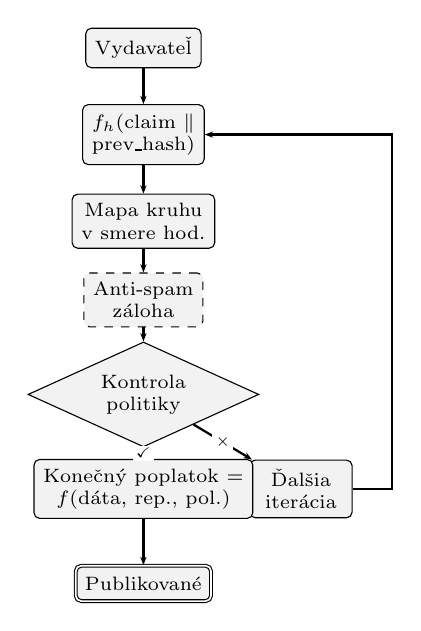
\begin{tikzpicture}[
    box/.style={draw, rounded corners=2pt, minimum width=1.3cm, minimum height=0.45cm, align=center, font=\scriptsize, fill=black!5},
    dec/.style={draw, diamond, aspect=2.2, minimum width=0.9cm, align=center, font=\scriptsize, fill=black!5},
    arr/.style={-{Stealth[length=3pt]}, thick},
    lbl/.style={font=\tiny, fill=white, inner sep=1pt}
]
\node[box] (iss) at (0,0) {Vydavateľ};
\node[box] (hash) at (0,-1.1) {$f_h$(claim $\|$\\prev\_hash)};
\node[box] (ring) at (0,-2.2) {Mapa kruhu\\v smere hod.};
\node[box, dashed] (spam) at (0,-3.2) {Anti-spam\\záloha};
\node[dec] (check) at (0,-4.4) {Kontrola\\politiky};
\node[box] (rej) at (2,-5.6) {Ďalšia\\iterácia};
\node[box] (fee) at (0,-5.6) {Konečný poplatok =\\$f$(dáta, rep., pol.)};
\node[box, double] (pub) at (0,-6.8) {Publikované};

\draw[arr] (iss) -- (hash);
\draw[arr] (hash) -- (ring);
\draw[arr] (ring) -- (spam);
\draw[arr] (spam) -- (check);
\draw[arr] (check) -- node[lbl] {$\times$} (rej);
\draw[arr] (check) -- node[lbl] {\checkmark} (fee);
\draw[arr] (fee) -- (pub);
\draw[arr] (rej.east) -- ++(0.5,0) |- (hash.east);
\end{tikzpicture}
\caption{Protokol výberu overovateľa. Anti-spam záloha je voliteľná a môže byť vratná. Konečný poplatok sa platí iba pri prijatí.}
\label{fig:verifier}
\end{figure}

Každé odmietnutie pripája úplnú odpoveď overovateľa (vrátane dôvodov a podmienok) k dokumentu tvrdenia, čím rozširuje jeho obsah. Z rozšíreného dokumentu sa nedeterministicky vypočíta nový hash, ktorý sa mapuje na inú pozíciu na kruhu a vyberá iného overovateľa. Zdokumentovanie úplnej cesty je povinné---vydavateľ nemôže predvídať ani ovplyvniť ďalšieho overovateľa. Ak overovateľ ignoruje žiadosť napriek kompatibilnej deklarovanej politike, svedkovia (ak sú prítomní) to zaznamenajú a vydavateľ môže pri konečnom publikovaní priložiť svedecké dôkazy.

\begin{figure}[ht]
\centering
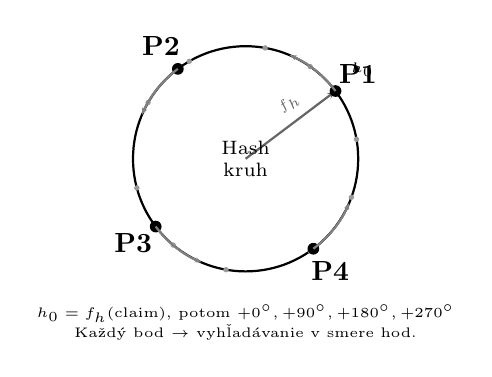
\begin{tikzpicture}[scale=0.65]
% Ring
\draw[thick] (0,0) circle (2.2cm);
% DID nodes on ring
\foreach \a in {10,55,80,120,150,195,230,260,305,340} {
  \fill[black!40] (\a:2.2) circle (1.5pt);
}
% Hash offset arrow pointing to initial position
\draw[-{Stealth[length=3pt]}, thick, black!60] (0,0) -- node[font=\tiny,above,sloped,pos=0.6] {$f_h$} (37:2.2);
\fill[black] (37:2.2) circle (2pt);
\node[font=\tiny,anchor=south west] at (37:2.35) {$h_0$};
% N=4 points offset from h0 by +0, +90, +180, +270
\foreach \offset/\l in {0/P1,90/P2,180/P3,270/P4} {
  \pgfmathsetmacro{\ang}{37+\offset}
  \node[fill=black, circle, inner sep=1.5pt] (p\offset) at (\ang:2.2) {};
  \node[font=\tiny,font=\bfseries] at (\ang:2.75) {\l};
  % clockwise search arc
  \draw[-{Stealth[length=2.5pt]}, thick, gray] (\ang:2.2) arc (\ang:\ang+30:2.2);
}
\node[font=\scriptsize, align=center] at (0,0) {Hash\\kruh};
\node[font=\tiny, align=center] at (0,-3.2) {$h_0 = f_h(\text{claim})$, potom $+0^{\circ},+90^{\circ},+180^{\circ},+270^{\circ}$\\Každý bod $\rightarrow$ vyhľadávanie v smere hod.};
\end{tikzpicture}
\caption{Viacbodový výber ($N{=}4$). Hash $h_0$ nastavuje posun; 4 body rovnomerne rozložené od $h_0$.}
\label{fig:multipoint}
\end{figure}

\subsection{Protokol svedka}

Rola \textbf{Svedka} poskytuje inkognito zodpovednosť za čestnosť overovateľa prostredníctvom kryptografického protokolu výzvových kódov:

\textbf{Krok W1.} Žiadateľ podpíše overovaciu žiadosť a odošle ju $N_w$ svedkom---kontaktom zo žiadateľovej sociálnej siete alebo špecializovaným poskytovateľom svedeckých služieb pracujúcim za poplatok.

\textbf{Krok W2.} Každý svedok $w_i$ podpíše celú podpísanú žiadosť, ponechá si pôvodný podpis $\sigma_i$ a vypočíta výzvový kód $c_i = h(\sigma_i)$. Výzvový kód sa pripojí k žiadosti.

\textbf{Krok W3.} Žiadosť, ktorá teraz nesie $N_w$ výzvových kódov, sa odošle overovateľovi. Overovateľ kódy vidí, ale \emph{nedokáže určiť}, kto sú svedkovia ani či kódy zodpovedajú skutočným podpisom.

\textbf{Krok W4 (čestný overovateľ).} Ak overovateľ odpovie podľa svojej deklarovanej politiky, výzvové kódy zostanú nepriehľadné. Svedkovia nie sú nikdy odhalení. Nepublikujú sa žiadne ďalšie dáta.

\textbf{Krok W5 (porušenie politiky).} Ak overovateľ poruší svoju politiku (ignoruje žiadosť, odpovedá nekonzistentne), žiadateľ drží pôvodné podpisy svedkov $\sigma_i$. Tie možno publikovať ako sprievodné dáta: ktokoľvek môže overiť $c_i = h(\sigma_i)$, čím sa dokáže, že svedok bol prítomný. Žiadateľ môže publikovať nezávisle---overovateľ už výzvové kódy vo svojej odpovedi podpísal.

\textbf{Vlastnosť blafovania.} Žiadateľ môže niektoré alebo všetky výzvové kódy nahradiť náhodnými hodnotami. Overovateľ nedokáže odlíšiť pravé kódy (kryté vysoko reputovanými autoritami) od šumu. Táto \emph{neistota} je vymáhacím mechanizmom: každá žiadosť nesie riziko, že nejaká rešpektovaná autorita prizerá inkognito. Náklady na udržiavanie tohto tlaku sú takmer nulové (generovanie náhodných čísel), zatiaľ čo potenciálne náklady nečestnosti pre overovateľa sú katastrofálne. Čestné správanie je stimulované aj bez skutočných svedkov.

\textbf{Autorita ako svedok.} Autorita, ktorá potvrdzuje tvrdenie, môže zväzať svedecké služby: ,,Potvrdzujem vaše tvrdenie a slúžim ako inkognito svedok počas overovania.`` Ide o prirodzený obchodný model---autorita už kontext má. Obe roly sú však logicky nezávislé.

\subsection{Princíp drahého radikalizmu}

Tri nákladové kanály sa kumulujú súčasne (Obr.~\ref{fig:radicalism}):

\textbf{Kanál 1: Náklady iterácie.} Každé odmietnutie vynúti novú iteráciu spotrebúvajúcu čas a zdroje. Lineárny rast.

\textbf{Kanál 2: Nabobtnávanie dokumentu.} Každá iterácia pridáva úplnú odpoveď overovateľa k dokumentu tvrdenia. Rast je lineárny, ale so základným posunom: počiatočný obsah (obsah tvrdenia, potvrdenie autoritou, kryptografické podpisy) už má netriviálnu veľkosť $B_0$. Celková veľkosť po $k$ iteráciách: $S(k) = B_0 + k \cdot \Delta$, kde $\Delta$ je priemerná veľkosť odpovede.

\textbf{Kanál 3: Riziková prirážka overovateľa.} Riziko je subjektívne. Overovateľ posudzuje, či deklarované politiky žiadajúceho DID kolidujú s vlastnými komerčnými, sociálnymi alebo politickými záujmami overovateľa. Prirážka môže exponenciálne eskalovať s vnímanou vzdialenosťou od ,,ideálu`` overovateľa: $P(d) = \alpha \cdot e^{\beta d}$, kde $d$ je subjektívna metrika vzdialenosti overovateľa. Za hranicou osobného ,,no-go`` môže overovateľ úplne odmietnuť.

\begin{figure}[ht]
\centering
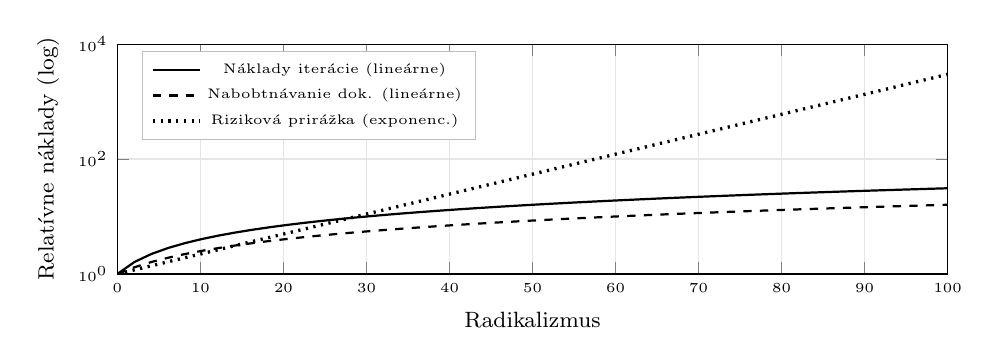
\begin{tikzpicture}
\begin{axis}[
    width=\columnwidth,
    height=4.5cm,
    xlabel={\footnotesize Radikalizmus},
    ylabel={\footnotesize Relatívne náklady (log)},
    ymode=log,
    xmin=0, xmax=100,
    ymin=1, ymax=10000,
    grid=major,
    grid style={gray!20},
    legend style={at={(0.03,0.97)},anchor=north west,font=\tiny,draw=gray!50},
    tick label style={font=\tiny},
    label style={font=\footnotesize},
]
\addplot[black, thick, domain=0:100, samples=50] {1 + 0.3*x};
\addlegendentry{Náklady iterácie (lineárne)}
\addplot[black, thick, dashed, domain=0:100, samples=50] {1 + 0.15*x};
\addlegendentry{Nabobtnávanie dok. (lineárne)}
\addplot[black, thick, dotted, line width=1.2pt, domain=0:100, samples=100] {exp(0.08*x)};
\addlegendentry{Riziková prirážka (exponenc.)}
\end{axis}
\end{tikzpicture}
\caption{Eskalácia nákladov naprieč tromi kanálmi. Riziková prirážka dominuje pri vysokom radikalizme.}
\label{fig:radicalism}
\end{figure}

Kľúčové je, že toto nie je cenzúra. Žiadne tvrdenie nie je zakázané. Systém oceňuje riziko (Tab.~\ref{tab:costs}).

\begin{table}[ht]
\centering
\caption{Porovnanie nákladov naprieč typmi tvrdení.}
\label{tab:costs}
\footnotesize
\begin{tabular}{@{}lcccc@{}}
\toprule
\textbf{Typ} & \textbf{Iter.} & \textbf{Dok} & \textbf{Poplatok} & \textbf{Spolu} \\
\midrule
Dôveryhodné & $k_{\min}$ & $B_0$ & $P_{\min}$ & Nízke \\
Kontroverzné & $k_{\text{med}}$ & $B_0{+}k\Delta$ & $\alpha e^{\beta d}$ & Stredné \\
Radikálne & $k_{\max}$ & $\gg B_0$ & $\gg P_{\min}$ & Veľmi vysoké \\
Podvodné & $\to\infty$ & --- & --- & Nepublikovateľné \\
\bottomrule
\end{tabular}
\end{table}

% ============================================================
% 6. REPUTATION AND RISK
% ============================================================
\section{Reputácia a hodnotenie rizika}

\subsection{Model hromadenia reputácie}

Reputácia vykazuje tri vlastnosti: \textbf{pomalé hromadenie} (postupný rast prostredníctvom konzistentného správania), \textbf{rýchle zničenie} (jediný podvod môže katastrofálne znížiť skóre) a \textbf{individuálne hodnotenie} (každá konzumujúca strana môže uplatniť vlastnú agregačnú funkciu).

\subsection{Reputované autority}

Reputovaná autorita preskúma tvrdenia a ak je spokojná, spolupodpíše ich---stavajúc svoju vlastnú reputáciu (Obr.~\ref{fig:authority}). Asymetria je zámerná: získavanie reputácie je pomalé (postupné $+\delta$ za každé čestné potvrdenie), zatiaľ čo jej strata je katastrofálna ($-\Delta \gg \delta$ za falošné potvrdenie; ilustratívne napr. $+2\%$ oproti $-70\%$). Optimálnou stratégiou je vždy odmietať podozrivé tvrdenia. Konkrétne hodnoty $\delta$ a $\Delta$ sú systémové parametre.

\begin{figure}[ht]
\centering
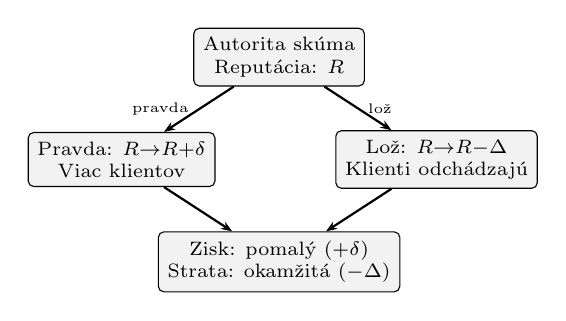
\begin{tikzpicture}[
    box/.style={draw, rounded corners=2pt, minimum width=2cm, minimum height=0.6cm, align=center, font=\scriptsize, fill=black!5},
    arr/.style={-{Stealth[length=4pt]}, thick}
]
\node[box] (exam) at (0,0) {Autorita skúma\\Reputácia: $R$};
\node[box] (true) at (-2,-1.3) {Pravda: $R{\to}R{+}\delta$\\Viac klientov};
\node[box] (false) at (2,-1.3) {Lož: $R{\to}R{-}\Delta$\\Klienti odchádzajú};
\node[box] (insight) at (0,-2.6) {Zisk: pomalý ($+\delta$)\\Strata: okamžitá ($-\Delta$)};

\draw[arr] (exam) -- node[left,font=\tiny] {pravda} (true);
\draw[arr] (exam) -- node[right,font=\tiny] {lož} (false);
\draw[arr] (true) -- (insight);
\draw[arr] (false) -- (insight);
\end{tikzpicture}
\caption{Reputovaná autorita---asymetrické stimuly.}
\label{fig:authority}
\end{figure}

\subsection{Viacrozmerná reputácia}

Reputácia nie je skalár, ale vektor naprieč viacerými dimenziami: finančná spoľahlivosť, osobná integrita, profesijná kompetentnosť, občianska angažovanosť a ďalšie (Obr.~\ref{fig:reputation-radar}). Rôzni poskytovatelia hodnotenia premietajú tento vektor odlišne v závislosti od kontextu---veriteľ uprednostňuje finančnú spoľahlivosť, zamestnávateľ profesijnú kompetentnosť, sused občianske správanie. Neexistuje jediné ,,správne`` reputačné skóre; iba perspektívy.

\begin{figure}[ht]
\centering
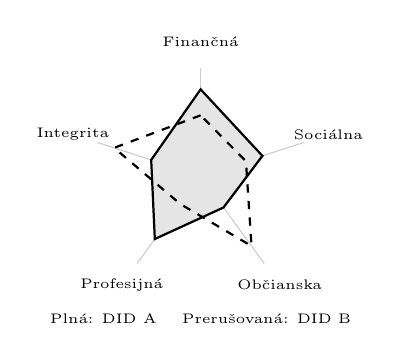
\begin{tikzpicture}[scale=0.55]
\foreach \a/\l in {90/Finančná,162/Integrita,234/Profesijná,306/Občianska,18/Sociálna} {
  \draw[gray!40] (0,0) -- (\a:2.5);
  \node[font=\tiny, align=center] at (\a:3.1) {\l};
  \foreach \r in {0.8,1.6,2.4} {
    \fill[black!15] (\a:\r) circle (0.5pt);
  }
}
\draw[thick, fill=black!10] (90:2.0) -- (162:1.2) -- (234:1.8) -- (306:0.9) -- (18:1.5) -- cycle;
\draw[thick, dashed] (90:1.4) -- (162:2.1) -- (234:0.8) -- (306:2.0) -- (18:1.1) -- cycle;
\node[font=\tiny] at (0,-3.3) {Plná: DID A \quad Prerušovaná: DID B};
\end{tikzpicture}
\caption{Viacrozmerné reputačné vektory. Rôzne DID vykazujú rôzne profily naprieč dimenziami.}
\label{fig:reputation-radar}
\end{figure}

\subsection{Demokratizované hodnotenie rizika}

RSN demokratizuje systematické hodnotenie rizika---schopnosť, ktorá je dnes sústredená vo finančných inštitúciách, ale použiteľná ďaleko za hranicami bankovníctva. Priemyselné konglomeráty posudzujúce spoľahlivosť dodávateľov, poisťovne oceňujúce behaviorálne riziko, due diligence pri fúziách a akvizíciách, odhad životnosti zariadení vo výrobe---kdekoľvek si riziko protistrany vyžaduje posúdenie, RSN poskytuje decentralizovanú, trhovo riadenú alternatívu. Trh interpretačných služieb prekladá surové viacrozmerné reputačné dáta na použiteľné súhrny, čím sprístupňuje hodnotenie protistrany ktorémukoľvek účastníkovi za marginálne náklady.

% ============================================================
% 7. CONSENSUS AND DISPUTE RESOLUTION
% ============================================================
\section{Konsenzus a riešenie sporov}

\subsection{Model decentralizovanej spravodlivosti}

RSN preformulúva spravodlivosť ako problém obojstranného vyjednávania. Hrozba trvalého, overiteľného poškodenia reputácie je účinnejším odstrašujúcim prostriedkom než súdne konanie, ktoré si poškodená strana nemôže dovoliť.

\subsection{Emergentný konsenzus}

Každý účastník si udržiava osobný prah zadosťučinenia. Agregovaný konsenzus siete vzniká ako štatistický priemer tisícov obojstranných vyjednávaní (Obr.~\ref{fig:consensus}). Reakcia výrazne nad konsenzom (barbarská) je drahá na publikovanie. Reakcia blízka konsenzu (proporcionálna) je lacná. Konsenzus nie je pravidlo---je to cenový signál.

\begin{figure}[ht]
\centering
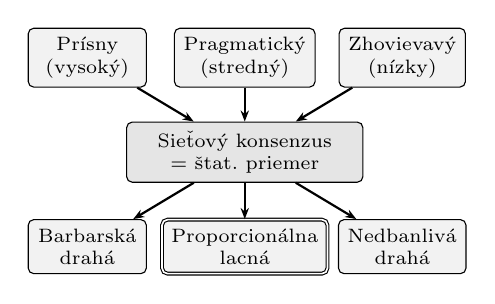
\begin{tikzpicture}[
    person/.style={draw, rounded corners=2pt, minimum width=1.5cm, minimum height=0.5cm, align=center, font=\scriptsize, fill=black!5},
    arr/.style={-{Stealth[length=4pt]}, thick}
]
\node[person] (a) at (-2,0) {Prísny\\(vysoký)};
\node[person] (b) at (0,0) {Pragmatický\\(stredný)};
\node[person] (c) at (2,0) {Zhovievavý\\(nízky)};
\node[person, fill=black!10, minimum width=3cm] (cons) at (0,-1.2) {Sieťový konsenzus\\= štat.\ priemer};
\node[person] (exp) at (-2,-2.4) {Barbarská\\drahá};
\node[person, double] (prop) at (0,-2.4) {Proporcionálna\\lacná};
\node[person] (neg) at (2,-2.4) {Nedbanlivá\\drahá};

\draw[arr] (a) -- (cons);
\draw[arr] (b) -- (cons);
\draw[arr] (c) -- (cons);
\draw[arr] (cons) -- (exp);
\draw[arr] (cons) -- (prop);
\draw[arr] (cons) -- (neg);
\end{tikzpicture}
\caption{Emergentný konsenzus z individuálnych prahov zadosťučinenia.}
\label{fig:consensus}
\end{figure}

\subsection{Kalibrácia trestu}

Každý držiteľ DID verejne deklaruje reakcie na konkrétne kategórie pochybenia. Neprimerane tvrdé alebo zhovievavé deklarácie priťahujú negatívne reputačné signály. Proporcionálne deklarácie sú prijímané bez trenia---samokalibračný trestný systém.

Deklarácie konsenzu samy podliehajú detekcii pokrytectva: deklaratívne zaviazať sa ku konsenzuálnej pozícii a pritom sa správať nekonzistentne predstavuje reputačný priestupok závažnejší než samotná odchýlka, keďže demonštruje úmyselné klamstvo.

\subsection{Delegovanie}

Všetky aktivity v rámci DID---s jednou výnimkou---môžu byť delegované na iný DID. \textbf{Rola subjektu---DID, o ktorého správaní tvrdenie je---nemôže byť delegovaná; je neprenosne viazaná na držiteľa identity, na ktorého sa tvrdenie vzťahuje.} Ostatné aktívne roly---Vydavateľ, Autorita, Svedok, Overovateľ---môžu byť prenesené na určený delegátsky DID, či už na overovanie, odosielanie tvrdení, účasť na konsenze alebo riešenie sporov. Delegovanie je kedykoľvek odvolateľné. To umožňuje špecializáciu (napr. profesionálne overovacie služby), pričom držiteľ si ponecháva konečnú kontrolu a zodpovednosť. Delegovanie sa uplatňuje naprieč celým systémom a je nevyhnutné pre škálovateľnosť.

\subsection{Od individuálnej morálky k emergentnej spoločenskej zmluve}

Deklarovaná politika každého DID predstavuje formalizáciu individuálnej morálky: čo držiteľ považuje za prijateľné, ako reaguje na konkrétne správanie, čo vyžaduje od protistrán. Tieto politiky nie sú vnútené návrhárom systému---sú zvolené každým účastníkom a vyjadrené v strojovo čitateľnej forme.

Táto formalizácia umožňuje trojfázový vznik. Po prvé, individuálna morálka je zakódovaná ako \textbf{politika}---sada deklarovaných pravidiel, prahov a reakčných funkcií, ktoré sa DID zaväzuje dodržiavať. Po druhé, agregát všetkých politík naprieč sieťou produkuje \textbf{emergentnú etiku}---štatisticky pozorovateľné normy, ktoré nenavrhol žiadny jednotlivý účastník, ale ktoré vznikajú z interakcie tisícov individuálnych morálnych pozícií~\cite{durkheim1893}. Po tretie, tieto emergentné etiky, vyjadrené ako zdieľané normy správania vymáhané prostredníctvom obojstranných cenových signálov, tvoria \textbf{merateľnú spoločenskú zmluvu}---nie teoretický konštrukt, ktorý nikto nepodpísal~\cite{rawls1971}, ale empiricky pozorovateľnú sadu pravidiel krytú skutočným správaním.

Tento proces zrkadlí zistenia z teórie morálnych základov~\cite{haidt2012}: ľudská morálka je intuitívna, pluralistická a kultúrne premenlivá. RSN nevyžaduje morálny konsenzus ako vstup; produkuje behaviorálny konsenzus ako výstup. Výsledná spoločenská zmluva nie je statická---vyvíja sa, ako sa účastníci pripájajú, odchádzajú a upravujú svoje politiky v reakcii na spätnú väzbu siete. Na rozdiel od klasickej teórie spoločenskej zmluvy je táto zmluva odvolateľná, pozorovateľná a vymáhateľná bez suveréna.

% ============================================================
% 8. ECONOMIC MODEL
% ============================================================
\section{Ekonomický model}

Predchádzajúce kapitoly opísali nástroj---overovacie mechanizmy RSN, nákladovú štruktúru a emergentný konsenzus. Táto kapitola opisuje metodiku uplatnenia tohto nástroja na fiškálny a správny prechod. Nástroj je univerzálny; nižšie uvedená metodika je jednou možnou aplikáciou.

\subsection{Štruktúra stimulov}

Reputácia ako kapitál vytvára priame stimuly pre čestné správanie. Za bežnej prevádzky si účastníci budujú reputáciu prirodzene prostredníctvom každodenných transakcií a splnených záväzkov. Primárny výdavok smeruje na \emph{negatívne} tvrdenia---zaznamenávanie škody spôsobenej inými. Táto asymetria stimuluje užitočné, spoľahlivé správanie: byť čestný nestojí nič navyše, zatiaľ čo byť škodlivý vytvára zdokumentovanú stopu, ktorú budú iní ochotní zaplatiť za jej uchovanie. Pokrytectvo---deklarovanie pravidiel bez ich dodržiavania---je najdrahším režimom zlyhania, keďže demonštruje úmyselné klamstvo.

\subsection{Paralelný fiškálny systém}

Tri komponenty umožňujú konkurenčný tlak: (1)~\textbf{jednoduchá daň}---jediná proporcionálna sadzba bez výnimiek, spočiatku marginálne pod existujúcou efektívnou sadzbou; (2)~\textbf{elektronická registrácia výdavkov (ESR)}---obrátenie českého modelu EET tak, aby občania dohliadali na štátne výdavky; (3)~\textbf{občanom riadené prideľovanie daní}---začínajúce na niekoľkých percentách v prvom roku a po desaťročí dosahujúce hocičo od nízkych dvojciferných hodnôt po úplnú migráciu na občanom riadený systém, v závislosti od miery prijatia. Skutočné tempo závisí od rýchlosti, akou vznikajú voľnotrhové alternatívy k štátnym službám, a od ochoty štátu spolupracovať na prechode; funkcia času nemusí byť lineárna a nie je dôvod stanovovať hornú hranicu toho, kam prijatie napokon môže dospieť.

% ============================================================
% 9. MIGRATION PATH
% ============================================================
\section{Migračná cesta}

Migrácia prebieha v troch fázach (Obr.~\ref{fig:migration}): \textbf{Fáza~1: Prekryv} (RSN ako informačná vrstva, štát je jediným poskytovateľom), \textbf{Fáza~2: Konkurencia} (RSN poskytuje funkčné alternatívy, súbežné používanie oboch systémov) a \textbf{Fáza~3: Prechod} (RSN prekonáva štátne ekvivalenty, dobrovoľná migrácia). Prechod je v každej fáze zvratný.

\begin{figure}[ht]
\centering
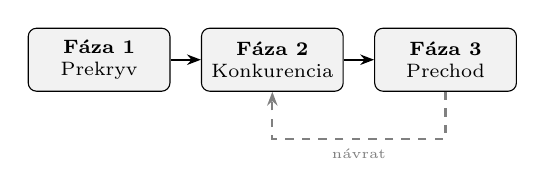
\begin{tikzpicture}[
    phase/.style={draw, rounded corners=3pt, minimum width=1.8cm, minimum height=0.8cm, align=center, font=\scriptsize, fill=black!5},
    arr/.style={-{Stealth[length=5pt]}, thick}
]
\node[phase] (p1) at (0,0) {\textbf{Fáza 1}\\Prekryv};
\node[phase] (p2) at (2.2,0) {\textbf{Fáza 2}\\Konkurencia};
\node[phase] (p3) at (4.4,0) {\textbf{Fáza 3}\\Prechod};

\draw[arr] (p1) -- (p2);
\draw[arr] (p2) -- (p3);
\draw[arr, dashed, gray] (p3.south) -- ++(0,-0.6) -| node[below,font=\tiny,pos=0.25] {návrat} (p2.south);
\end{tikzpicture}
\caption{Trojfázová migrácia---zvratná v každej fáze.}
\label{fig:migration}
\end{figure}

Primárnym tlakovým mechanizmom je fiškálny: keď podmienení daňoví poplatníci dosiahnu ,,ekonomicky významnú menšinu $X$``---skupinu dostatočne veľkú na to, aby represia voči nej spôsobila netriviálne ekonomické škody a občianska neposlušnosť sa stala vierohodnou hrozbou---štát vstupuje do vyjednávania. Na ilustráciu používame $X \approx 15\%$ HDP, ale skutočný prah závisí od konkrétnej ekonomiky.

% ============================================================
% 10. SECURITY ANALYSIS
% ============================================================
\section{Bezpečnostná analýza}

Uvažujeme päť kategórií protivníkov: jednotliví zlí aktéri, organizované skupiny, korporátni protivníci, protivníci na úrovni štátu a protivníci na úrovni protokolu.

\textbf{Odolnosť voči Sybil útoku}~\cite{douceur2002}. Budovanie reputácie vyžaduje trvalú, overiteľnú interakciu. Náklady na úspešný Sybil útok rastú lineárne s počtom falošných identít a kvadraticky s cieľovou úrovňou reputácie. Prevádzka viacerých DID paralelne je možná, ale zámerne drahá---každá identita si musí nezávisle nahromadiť reputáciu prostredníctvom skutočnej aktivity. V slobodných spoločnostiach tieto náklady odrádzajú od príležitostného zneužitia; v diktatúrach sa paralelné DID stávajú nástrojom prežitia umožňujúcim kompartmentalizovaný odpor, podzemnú koordináciu a bezpečnejšiu navigáciu na čiernom trhu.

\textbf{Obrana proti kolúzii.} Vzorce vzájomného potvrdzovania medzi uzavretými skupinami sú zistiteľné prostredníctvom analýzy sociálneho grafu. Agregačné funkcie reputácie diskontujú tvrdenia z tesne zhluknutých zdrojov.

\textbf{Protivník na úrovni štátu.} Onion smerovanie, absencia centralizovanej infraštruktúry a rozloženie roly overovateľa naprieč základňou účastníkov zabezpečujú, že potlačenie vyžaduje opatrenia neúmerné akémukoľvek prospechu.

\textbf{Súkromie vs.\ zodpovednosť.} Pseudonymita---stredná cesta medzi anonymitou a zverejnením identity---umožňuje DID hromadiť zmysluplnú reputáciu bez odhalenia reálnej identity držiteľa.

% ============================================================
% 11. PRIVACY
% ============================================================
\section{Aspekty súkromia}

Model súkromia RSN je postavený na pseudonymite. Držiteľ kontroluje zverejnenie identity: minimálne (čistý pseudonym), selektívne (prepojené konkrétne poverenia) alebo úplné (pridružená právna identita). Publikované tvrdenia sú trvalé---systém podporuje kontextuálnu opravu, ale nie vymazanie. Držiteľ môže opustiť kompromitovaný DID a začať odznova, čím sa vzdá nahromadenej reputácie.

% ============================================================
% 12. RELATED WORK
% ============================================================
\section{Súvisiaca práca}

Špecifikácia W3C DID Core~\cite{did2022} a sieť Ceramic~\cite{ceramic2023} poskytujú základ identity. EigenTrust~\cite{kamvar2003} demonštroval distribuovanú agregáciu reputácie bez centrálnej autority. SBT~\cite{weyl2022} zaviedli neprenosné sociálne tokeny. RSN sa líši dôrazom na ekonomické náklady ako filter kvality a svojím mechanizmom oceňovania radikalizmu.

DAO~\cite{buterin2014} a kvadratické hlasovanie~\cite{buterin2019} demonštrovali uskutočniteľnosť decentralizovanej správy. RSN odvodzuje konsenzus z obojstranných cenových vyjednávaní namiesto hlasovania.

Návrh čerpá z anarchokapitalistickej teórie~\cite{rothbard1973,hoppe2001} pre súkromné poskytovanie služieb, ale odkláňa sa v dvoch kľúčových ohľadoch: navrhuje pre zlomyseľnosť a odplatné impulzy namiesto predpokladania racionality a navrhuje postupný prechod namiesto revolúcie. Koncept emergentných spoločenských zmlúv má predchodcov v Hayekovej teórii spontánneho poriadku~\cite{hayek1973}.

\textbf{Anarcho-agorizmus.} RSN zdieľa významnú spoločnú pôdu s agoristickou protiekonomikou~\cite{konkin2006}---najmä dôraz na budovanie paralelných inštitúcií a dobrovoľnú výmenu. Agorizmus však má sklon predpokladať racionálny vlastný záujem ako dostatočný koordinačný mechanizmus a často mu chýba konkrétna migračná cesta z existujúcich štátnych štruktúr. RSN explicitne zahŕňa neracionálne behaviorálne sklony a poskytuje mechanizmus fiškálneho tlaku na postupný prechod.

\textbf{Meritokracia.} RSN môže predstavovať prvý funkčný opis toho, ako môže meritokracia~\cite{young1958} vzniknúť ako systémová vlastnosť namiesto slogana. Tradičné meritokratické systémy zlyhávajú, pretože vyžadujú centrálnu autoritu na definovanie a vymáhanie ,,zásluh``. V RSN zásluhy vznikajú z obojstranných hodnotení: tí, ktorí prinášajú hodnotu, hromadia reputáciu; žiadny výbor nerozhoduje, kto má zásluhy.

\textbf{Vlastníctvo ako privilégium.} RSN sa zásadne odkláňa od anarchokapitalistického a rakúsko-školského poňatia vlastníckych práv ako prirodzených a absolútnych. V rámci RSN je vlastníctvo \emph{privilégiom}---spoločenským uznaním, ktoré môže byť v extrémnych prípadoch odňaté komunitou, keď účastník zásadne poruší zdieľané normy (zrada, odmietnutie brániť komunitu v existenčnej kríze, systematické vykorisťovanie). Nejde o štátne vyvlastnenie, ale o odňatie spoločenského uznania sieťou obojstranných vzťahov.

% ============================================================
% 13. LIMITATIONS
% ============================================================
\section{Diskusia a obmedzenia}

\textbf{Studený štart.} Hodnota RSN závisí od sieťových efektov; skorí osvojitelia čelia obmedzenej hodnote, kým účasť nedosiahne prah. Avšak už od skorých fáz slúži sieť DID ako užitočný doplnkový zdroj informácií. Očakáva sa, že skoré hodnotenie reputácie a posudzovanie autorít sa budú postupne rozvíjať s rastúcou sofistikovanosťou.

\textbf{Ochrana proti parazitovaniu a kontrola prístupu.} Cieľové DID môžu ukladať odstupňované poplatky a obmedzenia prístupu pre dotazy od nízkoreputačných DID. Nejde o binárnu, ale o spojitú škálu: čím menej reputácie dotazujúci DID má, tým menej informácií dostane, tým dlhšie čaká a tým viac platí. Tento mechanizmus stimuluje skutočnú účasť namiesto pasívnej konzumácie.

\textbf{Nerovnosť prístupu.} Náklady na publikovanie tvrdení môžu odfiltrovať legitímne krivdy ekonomicky znevýhodnených účastníkov. Zmiernenie: každý účastník súčasne slúži ako potenciálny overovateľ (alebo túto rolu deleguje) a zarába overovacie poplatky. Za dostatočný časový horizont by sa neradikálny účastník mal priblížiť finančnej neutralite---príjem z overovania približne vyrovnáva náklady na publikovanie. Ide o štatistické očakávanie, nie o záruku.

\textbf{Nerovnosť reputácie.} Skorí osvojitelia hromadia výhody, ktoré môžu vytvárať bariéry pre neskorších príchodzích. Avšak hodnotenie reputácie vykonávajú poskytovatelia tretích strán, ktorí sa môžu rozhodnúť zmierniť výhodu prvého ťahu prostredníctvom svojich agregačných algoritmov. Byť prvý s dobrou reputáciou je legitímna komparatívna ekonomická výhoda---a to zámerne.

\textbf{Otvorené otázky.} Optimálne nákladové funkcie, štandardy agregácie, správa protokolu a interakcia s AI generovanými syntetickými reputačnými dátami zostávajú oblasťami pre budúcu prácu.

Tento článok netvrdí, že RSN prinesie optimálne výsledky za všetkých okolností. Tvrdí, že RSN predstavuje \emph{uskutočniteľnú} alternatívu---technicky implementovateľnú, ekonomicky sebestačnú a spoločensky kompatibilnú s ľudskými behaviorálnymi sklonmi tak, ako skutočne sú.

% ============================================================
% 14. CONCLUSION
% ============================================================
\section{Záver}

Tento článok predstavil Reputačnú sociálnu sieť, decentralizovaný protokol umožňujúci pseudonymnú, overiteľnú výmenu reputácie. Princíp drahého radikalizmu zabezpečuje, že podvodné tvrdenia sú cenovo vytláčané bez cenzúry. Navrhnutá migračná cesta umožňuje postupný, zvratný prechod z existujúcich inštitúcií. Návrh zahŕňa ľudskú povahu tak, ako je---vrátane malichernosti, zlomyseľnosti a túžby po odplatnom zadosťučinení---namiesto vyžadovania ideologickej premeny. Výsledkom nie je utópia, ale systém, kde je spravodlivosť dostupná, reputácia je zaslúžená a náklady na pochybenie nesie strana, ktorá ho spôsobila.

% ============================================================
% REFERENCES
% ============================================================
\bibliography{references}

\end{document}
